\section{Air, Combustion, Rusting and Fire Fighting}

\begin{multicols}{2}

\section*{Composition of Air}


\subsection{What is Air?}

\begin{center}
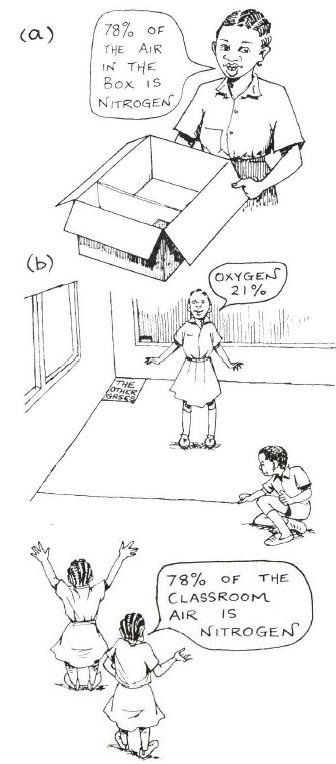
\includegraphics[width=0.45\textwidth]{./img/source/air-comp-1.jpg}
\end{center}

\begin{description*}
%\item[Subtopic:]{}
%\item[Materials:]{}
%\item[Setup:]{}
\item[Procedure:]{(a) To show the percentage by volume of
the different gases in air take a cardboard box of
about 50 cm $\times$ 50 cm $\times$ 50 cm and partition it
using cardboard pieces as shown in diagram (a)
according to the following figures: Nitrogen
78\%, Oxygen 2l\%, other 1\% (Argon 0.93\%,
other noble gases 0.002\%, carbon dioxide 0.03\%,
hydrogen 0.00l\%).
(b) The classroom can be imagined to be a box
with a certain volume of air and divided
accordingly by students as shown.}
%\item[Hazards:]{}
%\item[Questions:]{}
%\item[Observations:]{}
%\item[Theory:]{}
%\item[Applications:]{}
%\item[Notes:]{}
\end{description*}

\subsection{Gases in Air}

\begin{center}
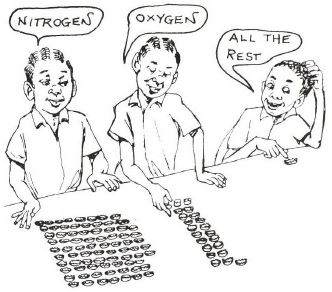
\includegraphics[width=0.4\textwidth]{./img/source/gases-in-air.jpg}
\end{center}

\begin{description*}
%\item[Subtopic:]{}
\item[Materials:]{Bottle tops/stones}
%\item[Setup:]{}
\item[Procedure:]{Collect a hundred bottle tops or
stones. Arrange in ten rows of ten. Each bottle
top represents one percent (by volume) of the
gases in the air. The bottle tops can then be
divided according to the percentages described
in the previous activity.}
%\item[Hazards:]{}
%\item[Questions:]{}
%\item[Observations:]{}
%\item[Theory:]{}
%\item[Applications:]{}
%\item[Notes:]{}
\end{description*}

%==================================================================================================%

\section*{Combustion}


\subsection{Requirements for Combustion}

\begin{center}
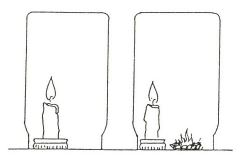
\includegraphics[width=0.4\textwidth]{./img/source/flame-extinguisher.jpg}
\end{center}

\begin{description*}
%\item[Subtopic:]{}
\item[Materials:]{2 glass jars, 2 candles, bottle caps, kerosene or spirit}
%\item[Setup:]{}
\item[Procedure:]{Place 1 jar over a lit candle and the other jar over both a candle and a kerosene or spirit flame in a bottle cap.}
%\item[Hazards:]{}
\item[Questions:]{Which candle flame goes out first?}
\item[Observations:]{The candle in the jar with the spirit burner goes out first.}
\item[Theory:]{Three elements are necessary for combustion: heat, fuel and oxygen. In the second jar, both the candle and spirit flame are consuming oxygen and so the oxygen gets depleted faster, extinguishing the flame.}
%\item[Applications:]{}
%\item[Notes:]{}
\end{description*}

\subsection{Rising Water}

\begin{center}
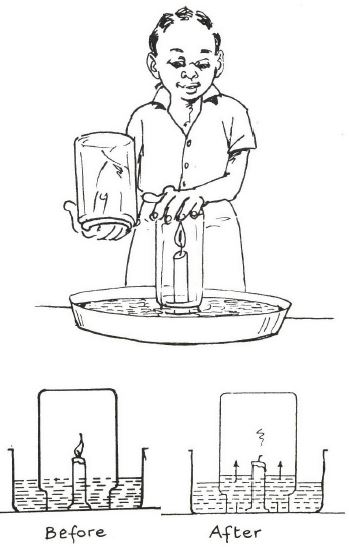
\includegraphics[width=0.4\textwidth]{./img/source/candle-water.jpg}
\end{center}

\begin{description*}
%\item[Subtopic:]{}
\item[Materials:]{Candle, dish, water, glass}
%\item[Setup:]{}
\item[Procedure:]{Place a candle in a dish fixing it securely with
melted wax. Fill the dish with water. Put glasses
of different sizes over the candle.}
%\item[Hazards:]{}
%\item[Questions:]{}
\item[Observations:]{The water rises to different levels after the flame goes out.}
\item[Theory:]{Once the glass is placed over the candle, the flame consumes the remainder of the oxygen in the glass, replacing it with carbon dioxide and other gases. The heating of the gases causes expansion and bubbles come out of the jar. This is followed by their subsequent cooling and contraction, which reduces the volume of gas inside the glass and allows water to enter.}
%\item[Applications:]{}
%\item[Notes:]{}
\end{description*}

\subsection{\texorpdfstring{\ce{H_2O}}{H_2O} as a Product of \hfill \\ Combustion} % Pic from elsewhere??? condensation

%\begin{center}
%\includegraphics[width=0.4\textwidth]{./img/.jpg}
%\end{center}

\begin{description*}
%\item[Subtopic:]{}
\item[Materials:]{Glass jar/plastic bottle, water, candle}
%\item[Setup:]{}
\item[Procedure:]{Fill the bottle with water and hold it just above a lit candle, far enough so that it does not burn.}
%\item[Hazards:]{}
%\item[Questions:]{}
\item[Observations:]{After a minute or two, condensation forms on the outside of the container, showing that water is a product of combustion.}
%\item[Theory:]{}
%\item[Applications:]{}
%\item[Notes:]{}
\end{description*}

\columnbreak

\subsection{\texorpdfstring{\ce{CO_2}}{CO_2} as a Product of \hfill \\ Combustion}

\begin{center}
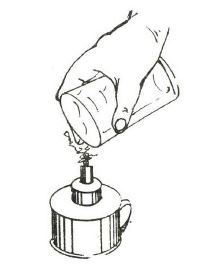
\includegraphics[width=0.4\textwidth]{./img/source/co2-extinguisher.jpg}
\end{center}

\begin{description*}
%\item[Subtopic:]{}
\item[Materials:]{Tall glass, wood ash, dilute acid, match, candle}
%\item[Setup:]{}
\item[Procedure:]{Place some wood ash in a tall glass and add some dilute acid. Drop a lit match into the glass and wait for it to stop burning. Now pour the glass over a lit candle.}
%\item[Hazards:]{}
%\item[Questions:]{}
\item[Observations:]{Pouring the glass puts out the candle flame.}
\item[Theory:]{The carbon dioxide produced stays in the
glass since it is denser than air. Carbon dioxide
extinguishes flames since it does not support
combustion.}
\item[Applications:]{Fire extinguishers}
%\item[Notes:]{}
\end{description*}

\subsection{Burning Money}

%\begin{center}
%\includegraphics[width=0.4\textwidth]{./img/.jpg}
%\end{center}

\begin{description*}
%\item[Subtopic:]{}
\item[Materials:]{Methylated spirits, water, container, matches, paper money, clothespin}
%\item[Setup:]{}
\item[Procedure:]{Make a mixture of 3 parts methylated spirits and 2 parts water. Soak the money in the mixture. Remove with a clothespin and light it with a match. After about 5 seconds drop the money into the extra water.}
%\item[Hazards:]{}
%\item[Questions:]{}
\item[Observations:]{The money appears to burn but remains intact.}
\item[Theory:]{The ethanol in the methylated spirit burns at a low temperature while the water protects the bill from combusting. However, if there is a lot of ethanol and it burns for a long time, the water will evaporate away and the bill will start burning.}
%\item[Applications:]{}
%\item[Notes:]{}
\end{description*}

%==================================================================================================%

\section*{Firefighting}


\subsection{Putting Out Fires} % LASM 37

\begin{center}
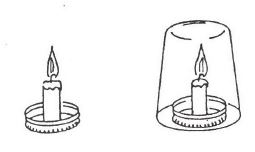
\includegraphics[width=0.4\textwidth]{./img/source/fire-fighting.jpg}
\end{center}

\begin{description*}
%\item[Subtopic:]{}
\item[Materials:]{Bottle caps, ethanol, kerosene, water, matches, sand, glass jar}
%\item[Setup:]{}
\item[Procedure:]{Put a small amount of ethanol into a bottle cap and light it with a match. Pour water onto the flame. Repeat using a handful of sand and then an inverted glass over the flame. Now add a small amount of kerosene to a bottle cap. Repeat the above methods, but add water \emph{carefully} using a syringe near the base of the flame. Repeat the steps for a burning piece of paper.}
\item[Hazards:]{Perform these tests on a laboratory floor, not a wooden table or desk.}
%\item[Questions:]{}
\item[Observations:]{The ethanol and paper flames are extinguished in all 3 cases. However, adding water to the kerosene \emph{does not} extinguish it.}
\item[Theory:]{Overturning a glass jar deprives the flames of oxygen and thus extinguishes them. A kerosene fire can NOT be extinguished by water because water is immiscible with kerosene, and it only causes the fire to spread.}
%\item[Applications:]{}
%\item[Notes:]{}
\end{description*}

\vfill
\columnbreak

\subsection{Making a Fire Extinguisher}

\begin{center}
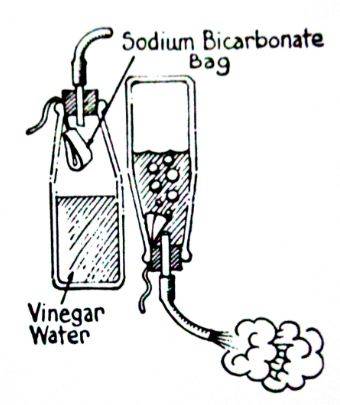
\includegraphics[width=0.35\textwidth]{./img/fire-extinguisher.jpg}
\end{center}

\begin{description*}
%\item[Subtopic:]{}
\item[Materials:]{Bottle, tea bag, bicarbonate of soda, vinegar, water, plastic tube, super glue}
\item[Setup:]{Empty a tea bag and fill it with sodium bicarbonate. Suspend it in a bottle half-filled with a vinegar-water solution. Poke a hole in the cap and insert a plastic tube. Make sure it is sealed using super glue or clay.}
\item[Procedure:]{Invert the bottle and use the tube to direct the spray at a lit candle.}
%\item[Hazards:]{}
%\item[Questions:]{}
%\item[Observations:]{}
\item[Theory:]{The reaction produces carbon dioxide gas which extinguishes flames. This is how fire extinguishers eliminate flames.}
%\item[Applications:]{}
%\item[Notes:]{}
\end{description*}

\vfill
\columnbreak

%==================================================================================================%

\section*{Rusting}


\subsection{Conditions for Rusting}

\begin{center}
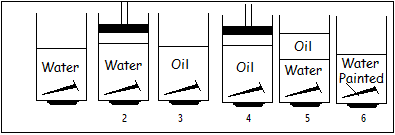
\includegraphics[width=0.4\textwidth]{./img/rusting-nails-6.png}
\end{center}

\begin{description*}
%\item[Subtopic:]{}
\item[Materials:]{6 syringes, 6 nails, water, oil, paint}
\item[Setup:]{Seal the bottoms of the syringes by melting the plastic.}
\item[Procedure:]{Place a nail in each syringe. Paint the final nail. Fill the syringes as shown, closing some of them with their plungers. Observe the nails over time and note which ones show rusting.}
%\item[Hazards:]{}
%\item[Questions:]{}
\item[Observations:]{Syringe 1 should show rusting, while the others do not.}
\item[Theory:]{Syringe 1 is the control - both water and oxygen react with the nail. In syringe 2, no oxygen is available. In syringe 3, there is no water and oil makes it difficult for oxygen to reach the nail. In syringe 4, neither water nor oxygen are present. In syringe 5, water is available, but the layer of oil prevents oxygen from reaching it since oxygen does not travel easily through oil. In syringe 6, painting covers the iron surface, so there is no iron to produce rusting.}
%\item[Applications:]{}
%\item[Notes:]{}
\end{description*}

\subsection{Rusting of Steel Wool} % VSO 65

\begin{center}
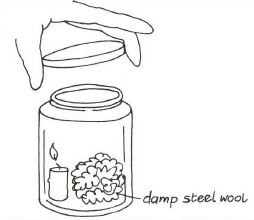
\includegraphics[width=0.35\textwidth]{./img/vso/rusting-steel-wool.jpg}
\end{center}

\begin{description*}
%\item[Subtopic:]{}
\item[Materials:]{Steel wool, candle, 2 glass containers}
%\item[Setup:]{}
\item[Procedure:]{Wet the steel wool and place some in each container. Seal one
container. Place a lighted candle in the other container. When the
candle has burnt for several minutes seal the container with a lid. The
candle will go out eventually. Leave both containers for 2 days. }
%\item[Hazards:]{}
%\item[Questions:]{}
\item[Observations:]{The
steel wool in the container with the candle should not rust as much
because oxygen has been removed by the candle.}
%\item[Theory:]{}
%\item[Applications:]{}
%\item[Notes:]{}
\end{description*}

\columnbreak

\subsection{Rusty Nails}

\begin{center}
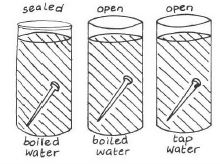
\includegraphics[width=0.4\textwidth]{./img/vso/rusty-nails.jpg}
\end{center}

\begin{description*}
%\item[Subtopic:]{}
\item[Materials:]{3 containers, 2 nails, boiled water, tap water}
%\item[Setup:]{}
\item[Procedure:]{Place a nail in each of the
containers and leave for a day.}
%\item[Hazards:]{}
%\item[Questions:]{}
\item[Observations:]{The only nail which does not rust
is the one in the sealed jar of
boiled water.}
\item[Theory:]{Boiling the water
removes the oxygen and sealing it
prevents oxygen from the air
dissolving in it.}
%\item[Applications:]{}
%\item[Notes:]{}
\end{description*}

\subsection{Preventing Rusting} % VSO 65

\begin{center}
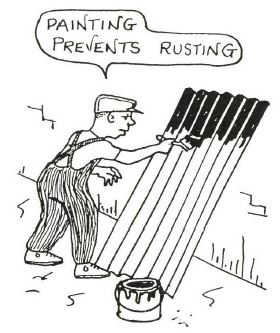
\includegraphics[width=0.4\textwidth]{./img/source/rusting-prevent.jpg}
\end{center}

\begin{description*}
%\item[Subtopic:]{}
\item[Materials:]{tin can, oil}
%\item[Setup:]{}
\item[Procedure:]{Make 2 large scratches on the surface of a tin can (not an aluminium
can often used for drinks). Put a thin layer of oil onto one scratch.
Leave the tin exposed to the air for a few days. Note which scratch
rusts.}
%\item[Hazards:]{}
%\item[Questions:]{}
\item[Observations:]{The scratch not covered in oil rusts, while the other does not.}
\item[Theory:]{Oil prevents water and oxygen from reaching the surface of metal, and so no rusting occurs.}
\item[Applications:]{Machine parts often cannot be protected by painting or other means so they are regularly oiled.}
%\item[Notes:]{}
\end{description*}

%==================================================================================================%


\end{multicols}

\pagebreak